\documentclass[a4paper,12pt]{article}

\usepackage[utf8]{inputenc}
\usepackage[russian]{babel}
\usepackage[top=1.8cm, bottom=1.8cm, left=1.8cm, right=1.8cm]{geometry}
\usepackage{amsmath, amsfonts, amssymb}
\usepackage{graphicx}
\usepackage{booktabs}
\usepackage{float}
\usepackage{caption}

\begin{document}
	
	\begin{center}
		\textbf{\Large Отчет по заданию 1}\\
		\textbf{\large (кастомное разложение)}
	\end{center}
	
	\vspace{0.3em}
	\noindent \textbf{Выполнил:} Оплакаская А.М., группа 26152. \\
	\textbf{Вариант 14.}
	
	\vspace{0.7em}
	\noindent \textbf{Описание задания:} В качестве базиса полиномиального пространства использовались полиномы Лежандра $P_j(\varepsilon)$ ($j = 0, \dots, N$). Численное решение переопределенной СЛАУ $A c \approx b$ реализовано тремя методами:
	\begin{enumerate}
		\item Метод НУ с факторизацией Холецкого;
		\item QR-алгоритм на основе метода вращений Гивенса с выбором главного элемента по столбцам;
		\item \textbf{Самостоятельно реализованный метод SVD} без вызова сторонних библиотечных функций разложения.
	\end{enumerate}
	Программа написана на языке \textbf{Rust}.
	
	\vspace{0.7em}
	\noindent \textbf{Тестирование алгоритмов на матрице $3 \times 2$:} \\
	Для матрицы $A = \begin{pmatrix} 1 & 2 \\ 3 & 4 \\ 5 & 6 \end{pmatrix}$ получены следующие результаты:
	\begin{itemize}
		\item \textbf{QR:}
		\[
		Q = \begin{pmatrix} 
			0.1690 & 0.8971 & 0.4082 \\ 
			0.5071 & 0.2760 & -0.8165 \\ 
			0.8452 & -0.3450 & 0.4082 
		\end{pmatrix}, \quad
		R = \begin{pmatrix} 
			5.9161 & 7.4374 \\ 
			0.0000 & 0.8281 \\ 
			0.0000 & 0.0000 
		\end{pmatrix}
		\]
		\item \textbf{Кастомный SVD:} сингулярные числа $\sigma_1 = 9.5255$, $\sigma_2 = 0.5143$. Восстановленная матрица $U \Sigma V^T = A$ совпадает с исходной с машинной точностью ($10^{-15}$).
	\end{itemize}
	
	\vspace{0.5em}
	\noindent \textbf{Таблица 1.} Результаты расчетов для данных 2 (\texttt{data\_2.txt})
	\begin{table}[H]
		\centering
		\resizebox{\textwidth}{!}{
			\begin{tabular}{|c|c|c|c|c|c|c|c|c|}
				\hline
				$N$ & $\text{cond}_2(A^T A)$ & NRMSE НУ & $t_{\text{НУ}}$, с & $\text{cond}_2(A)$ & NRMSE QR & $t_{\text{QR}}$, с & NRMSE SVD & $t_{\text{SVD}}$, с \\ \hline
				0  & 1.00e+0  & 2.88e-1 & 0.00026 & 1.00e+0 & 2.88e-1 & 0.00045 & 2.88e-1 & 0.00022 \\ \hline
				1  & 3.06e+2  & 1.14e-2 & 0.00029 & 1.75e+1 & 1.14e-2 & 0.00092 & 1.14e-2 & 0.00032 \\ \hline
				2  & 8.25e+4  & 6.72e-4 & 0.00039 & 2.87e+2 & 6.72e-4 & 0.00167 & 6.72e-4 & 0.00108 \\ \hline
				3  & 3.21e+7  & 6.69e-4 & 0.00044 & 5.67e+3 & 6.69e-4 & 0.00156 & 6.69e-4 & 0.00177 \\ \hline
				4  & 1.25e+10 & 6.66e-4 & 0.00060 & 1.12e+5 & 6.66e-4 & 0.00240 & 6.66e-4 & 0.00277 \\ \hline
				5  & 5.33e+12 & 4.41e-4 & 0.00056 & 2.31e+6 & 4.41e-4 & 0.00298 & 4.41e-4 & 0.00350 \\ \hline
				6  & 2.00e+15 & 2.51e-4 & 0.00067 & 4.75e+7 & 2.47e-4 & 0.00293 & 2.47e-4 & 0.00327 \\ \hline
				7  & 5.72e+16 & 2.39e-4 & 0.00044 & 1.00e+9 & 2.36e-4 & 0.00352 & 2.36e-4 & 0.00798 \\ \hline
				8  & 5.37e+17 & 2.99e-4 & 0.00167 & 2.10e+10& 2.03e-4 & 0.00621 & 2.03e-4 & 0.01479 \\ \hline
				9  & 1.33e+17 & Сбой (НУ)& ---     & 4.50e+11& 1.80e-4 & 0.00710 & 1.80e-4 & 0.01183 \\ \hline
				10 & 1.49e+17 & Сбой (НУ)& ---     & 9.52e+12& 1.67e-4 & 0.00668 & 1.67e-4 & 0.01841 \\ \hline
			\end{tabular}
		}
	\end{table}
	
	\noindent \textbf{Таблица 2.} Результаты расчетов для данных 4 (\texttt{data\_4.txt})
	\begin{table}[H]
		\centering
		\resizebox{\textwidth}{!}{
			\begin{tabular}{|c|c|c|c|c|c|c|c|c|}
				\hline
				$N$ & $\text{cond}_2(A^T A)$ & NRMSE НУ & $t_{\text{НУ}}$, с & $\text{cond}_2(A)$ & NRMSE QR & $t_{\text{QR}}$, с & NRMSE SVD & $t_{\text{SVD}}$, с \\ \hline
				0  & 1.00e+0  & 3.32e-1  & 0.00005 & 1.00e+0 & 3.32e-1  & 0.00008 & 3.32e-1  & 0.00004 \\ \hline
				1  & 1.92e+1  & 8.30e-2  & 0.00006 & 4.39e+0 & 8.30e-2  & 0.00016 & 8.30e-2  & 0.00007 \\ \hline
				2  & 4.00e+2  & 8.81e-15 & 0.00009 & 2.00e+1 & 2.15e-15 & 0.00025 & 3.93e-16 & 0.00015 \\ \hline
				3  & 1.07e+4  & 4.83e-14 & 0.00011 & 1.04e+2 & 2.17e-15 & 0.00039 & 6.17e-16 & 0.00028 \\ \hline
				4  & 3.10e+5  & 2.79e-13 & 0.00012 & 5.57e+2 & 1.99e-15 & 0.00052 & 1.27e-15 & 0.00050 \\ \hline
				5  & 9.36e+6  & 2.02e-12 & 0.00012 & 3.06e+3 & 2.04e-15 & 0.00062 & 7.83e-16 & 0.00093 \\ \hline
				6  & 2.88e+8  & 1.10e-11 & 0.00013 & 1.70e+4 & 2.05e-15 & 0.00089 & 6.99e-16 & 0.00106 \\ \hline
				7  & 9.03e+9  & 6.01e-11 & 0.00010 & 9.50e+4 & 2.03e-15 & 0.00076 & 7.28e-16 & 0.00122 \\ \hline
				8  & 2.86e+11 & 3.29e-10 & 0.00020 & 5.34e+5 & 1.93e-15 & 0.00102 & 9.69e-16 & 0.00178 \\ \hline
				9  & 9.12e+12 & 1.80e-9  & 0.00025 & 3.02e+6 & 2.05e-15 & 0.00136 & 1.22e-15 & 0.00261 \\ \hline
				10 & 2.97e+14 & 1.01e-8  & 0.00017 & 1.71e+7 & 2.09e-15 & 0.00112 & 5.01e-16 & 0.00273 \\ \hline
			\end{tabular}
		}
	\end{table}
	
	\noindent \textbf{Таблица 3.} Результаты расчетов для данных 5 (\texttt{data\_5.txt})
	\begin{table}[H]
		\centering
		\resizebox{\textwidth}{!}{
			\begin{tabular}{|c|c|c|c|c|c|c|c|c|}
				\hline
				$N$ & $\text{cond}_2(A^T A)$ & NRMSE НУ & $t_{\text{НУ}}$, с & $\text{cond}_2(A)$ & NRMSE QR & $t_{\text{QR}}$, с & NRMSE SVD & $t_{\text{SVD}}$, с \\ \hline
				0  & 1.00e+0  & 2.94e-1  & 0.00006 & 1.00e+0 & 2.94e-1  & 0.00009 & 2.94e-1  & 0.00006 \\ \hline
				1  & 1.92e+1  & 2.76e-2  & 0.00007 & 4.39e+0 & 2.76e-2  & 0.00019 & 2.76e-2  & 0.00008 \\ \hline
				2  & 4.00e+2  & 2.32e-3  & 0.00012 & 2.00e+1 & 2.32e-3  & 0.00029 & 2.32e-3  & 0.00018 \\ \hline
				3  & 1.07e+4  & 1.46e-4  & 0.00013 & 1.04e+2 & 1.46e-4  & 0.00046 & 1.46e-4  & 0.00036 \\ \hline
				4  & 3.10e+5  & 7.32e-6  & 0.00020 & 5.57e+2 & 7.32e-6  & 0.00058 & 7.32e-6  & 0.00059 \\ \hline
				5  & 9.36e+6  & 3.06e-7  & 0.00013 & 3.06e+3 & 3.06e-7  & 0.00066 & 3.06e-7  & 0.00075 \\ \hline
				6  & 2.88e+8  & 1.09e-8  & 0.00008 & 1.70e+4 & 1.09e-8  & 0.00058 & 1.09e-8  & 0.00076 \\ \hline
				7  & 9.03e+9  & 3.43e-10 & 0.00009 & 9.50e+4 & 3.43e-10 & 0.00068 & 3.43e-10 & 0.00123 \\ \hline
				8  & 2.86e+11 & 8.53e-11 & 0.00017 & 5.34e+5 & 9.54e-12 & 0.00095 & 9.54e-12 & 0.00179 \\ \hline
				9  & 9.12e+12 & 4.39e-10 & 0.00023 & 3.02e+6 & 2.39e-13 & 0.00138 & 2.39e-13 & 0.00285 \\ \hline
				10 & 2.97e+14 & 2.32e-9  & 0.00026 & 1.71e+7 & 5.52e-15 & 0.00157 & 5.53e-15 & 0.00350 \\ \hline
			\end{tabular}
		}
	\end{table}
	
	\begin{figure}[H]
		\centering
		% Файл data_5.png генерируется скриптом plot.py
		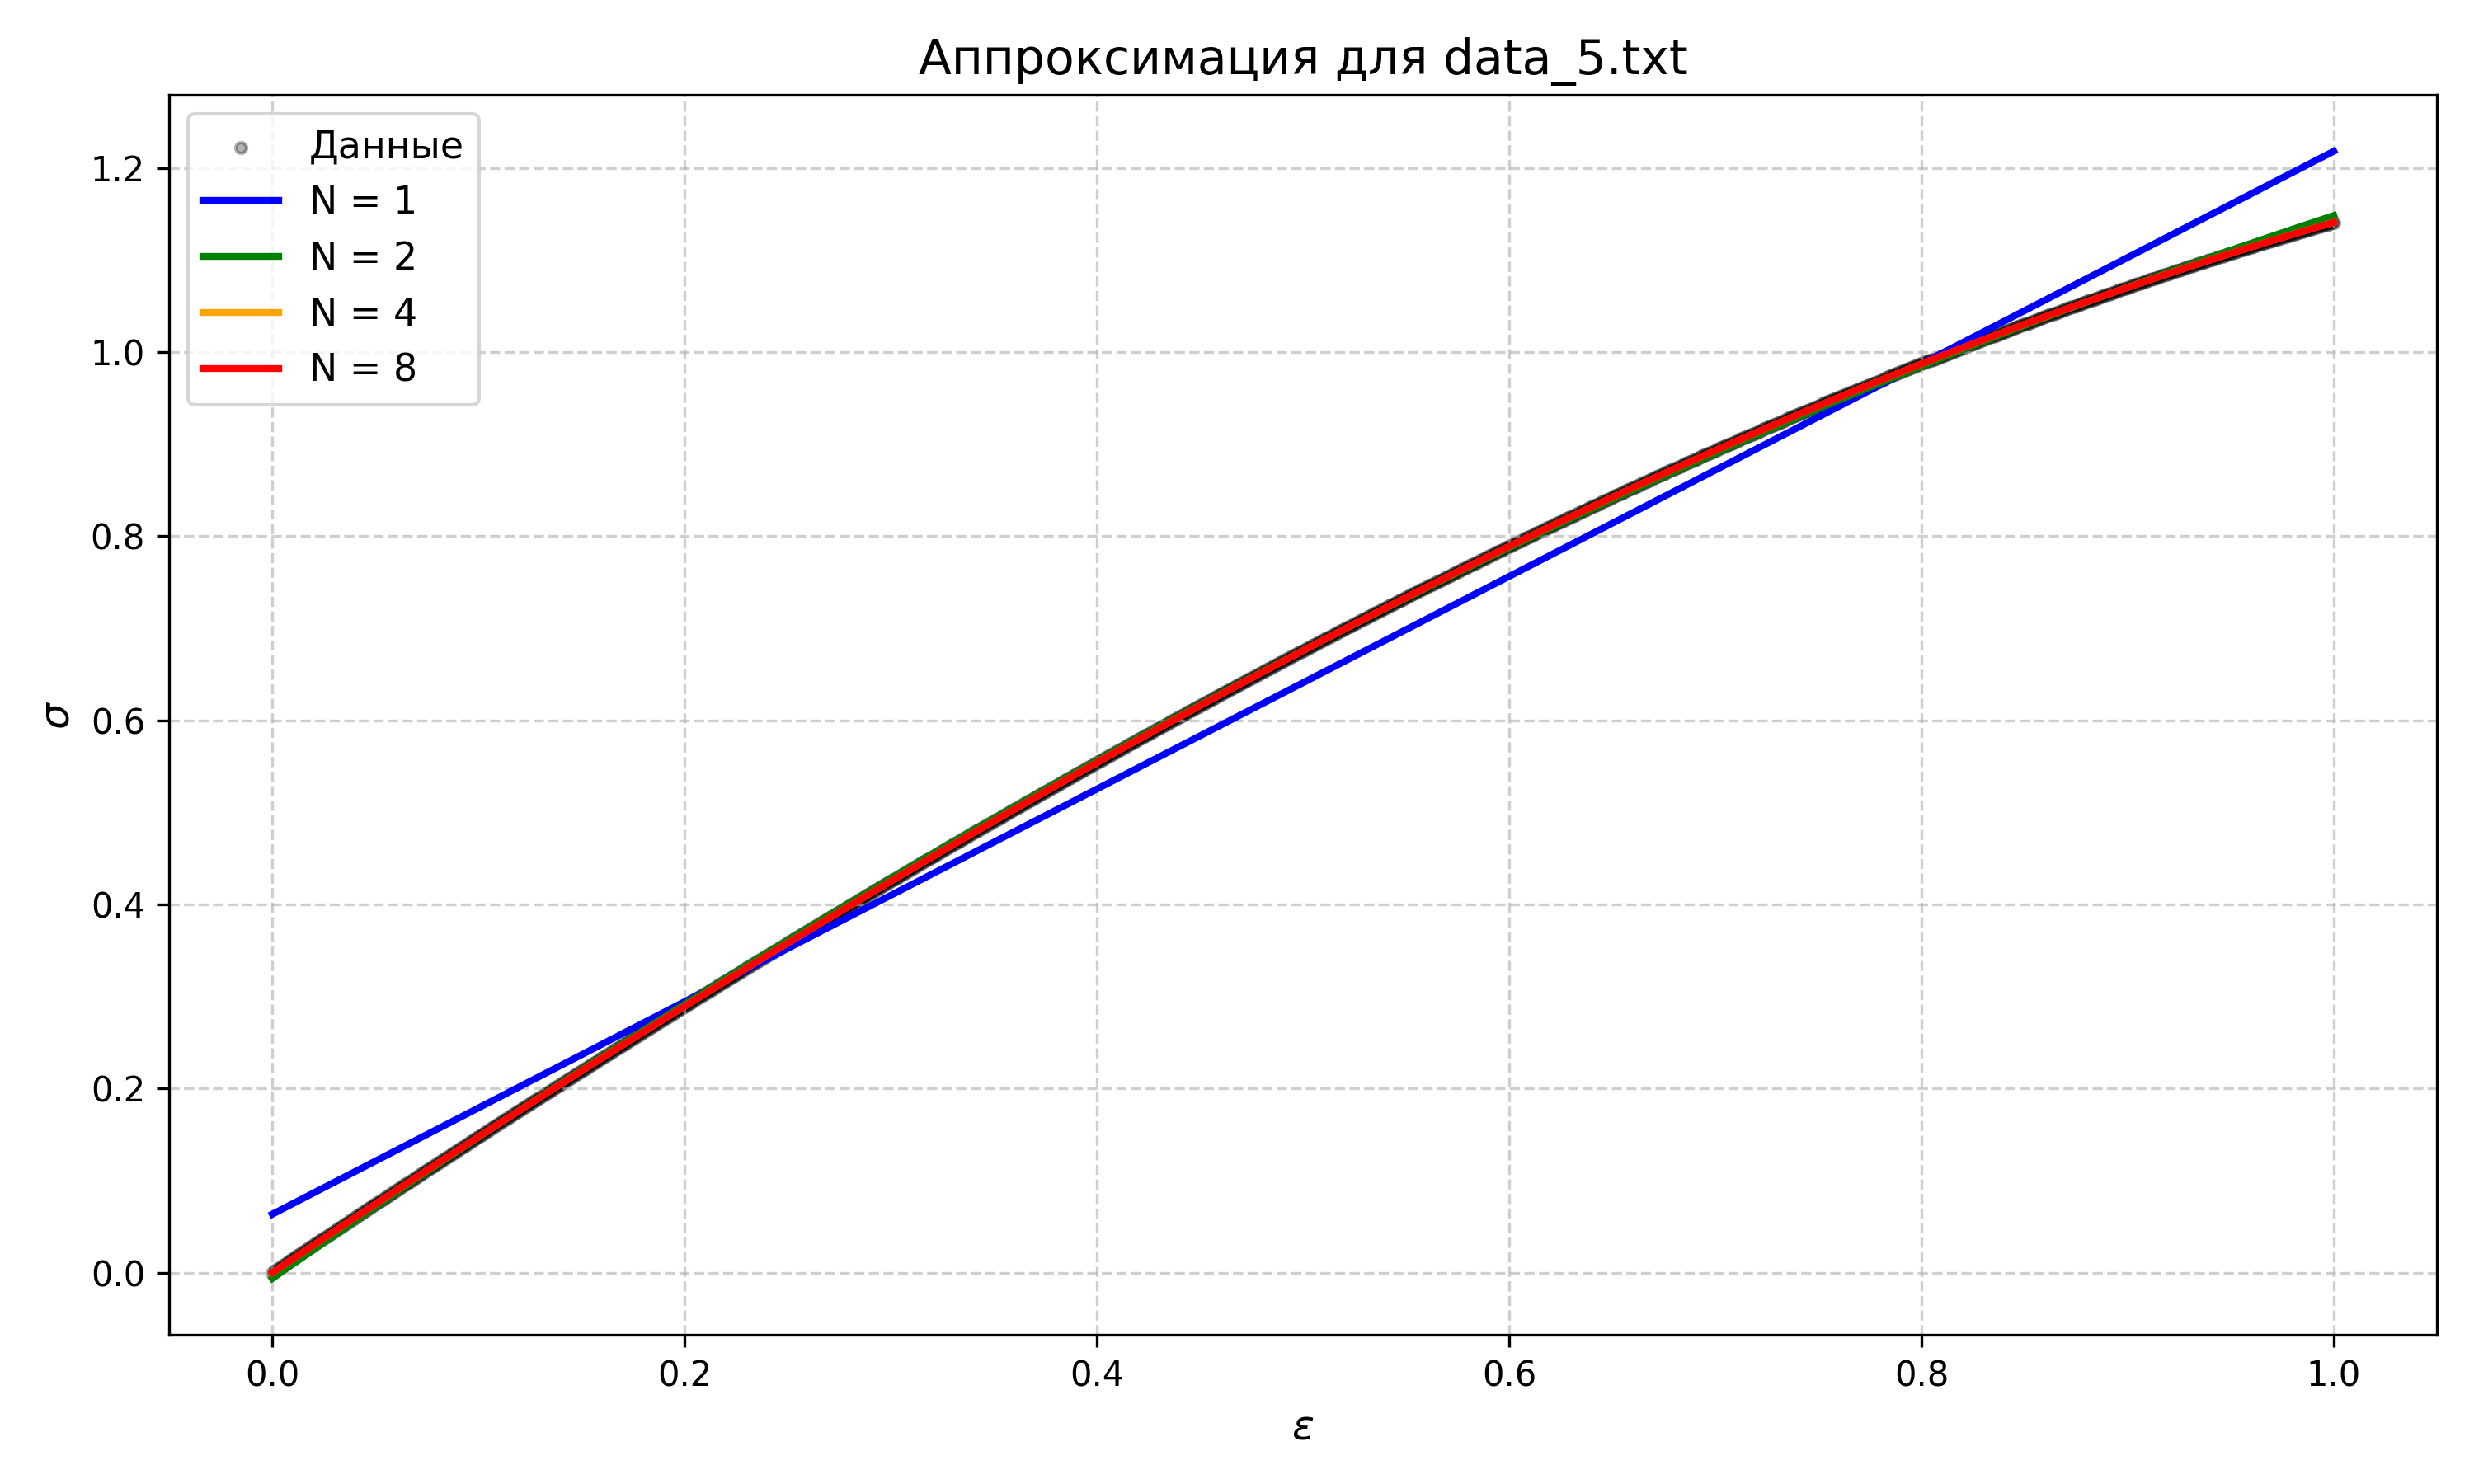
\includegraphics[width=0.85\textwidth]{data_5.png}
		\caption{Аппроксимация данных полиномами Лежандра для \texttt{data\_5.txt}}
	\end{figure}
	
	\vspace{0.5em}
	\noindent \textbf{Выводы и сравнительный анализ трех методов:}
	
	\begin{enumerate}
		\item \textbf{Сравнение чисел обусловленности:} Экспериментально подтверждено квадратичное соотношение $\text{cond}_2(A^T A) = [\text{cond}_2(A)]^2$. В Таблице 1 для данных 2 при $N \ge 7$ матрица $A^T A$ выходит за пределы машинного нуля, в результате чего метод Холецкого на шагах $N = 9, 10$ падает из-за потери численной положительной определенности. 
		
		\item \textbf{Сравнение QR и кастомного SVD:} 
		Оба метода показали устойчивость:
		\begin{itemize}
			\item На данных 4 при $N = 2$ невязка падает до машинного нуля, что говорит о параболической зависимости исходного набора точек.
			\item На данных 5 оба метода достигают предельной точности $5.5 \cdot 10^{-15}$ при $N = 10$, в то время как метод НУ откатывается до $2.3 \cdot 10^{-9}$ из-за накопления погрешностей.
			\item Касотмный SVD на основе псевдообращения показал бОльшую точность даже незначительно опережая QR на данных 4.
		\end{itemize}
		
		\item \textbf{Сравнение времени работы:} 
		Метод НУ является самым быстрым по времени расчета, т.к. решает СЛАУ малой размерности. Метод QR работает за время $t \sim 10^{-3}$ с. Кастомный SVD требует больше времени примерно на порядок, поскольку алгоритм вращений Якоби является итерационным процессом, требующим нескольких проходов по столбцам до достижения сходимости по норме. Однако эта вычислительная стоимость окупается абсолютной численной надежностью алгоритма.
	\end{enumerate}
	
\end{document}